\documentclass[a4paper, 14pt]{extarticle}
\usepackage[english,russian]{babel}
\usepackage[T1]{fontenc}
\usepackage[utf8]{inputenc}
\usepackage{fontspec}
\usepackage{indentfirst}
\usepackage{enumitem}
\usepackage{graphicx}
\usepackage[
  left=20mm,
  right=10mm,
  top=20mm,
  bottom=20mm
]{geometry}
\usepackage{parskip}
\usepackage{titlesec}
\usepackage{xurl}
\usepackage{hyperref}
\usepackage{float}
\usepackage[
  figurename=Рисунок,
  labelsep=endash,
  justification=centering
]{caption}
\usepackage[outputdir=build, newfloat]{minted}
\usepackage{chngcntr}

\selectlanguage{russian}

\hypersetup{
  colorlinks=true,
  linkcolor=black,
  filecolor=blue,
  urlcolor=blue,
}

\renewcommand*{\labelitemi}{---}
\setmainfont{Times New Roman}
\setmonofont{JetBrains Mono}[
  SizeFeatures={Size=11},
]

\newenvironment{code}{\captionsetup{type=figure}}{}
\BeforeBeginEnvironment{code}{\bigskip}
\AfterEndEnvironment{code}{\bigskip}

\setminted{
  fontsize=\footnotesize,
}

\setlength{\parskip}{6pt}

\setlength{\parindent}{1.25cm}
\setlist[itemize]{itemsep=0em,topsep=0em,parsep=0em,partopsep=0em,leftmargin=2.0cm,wide}
\setlist[enumerate]{itemsep=0em,topsep=0em,parsep=0em,partopsep=0em,leftmargin=2.0cm,wide}

\renewcommand{\thesection}{\indent\arabic{section}.}
\renewcommand{\thesubsection}{\indent\thesection\arabic{subsection}.}
\renewcommand{\thesubsubsection}{\indent\thesubsection\arabic{subsubsection}.}

\titleformat{\section}{\normalfont\bfseries}{\thesection}{0.5em}{}
\titleformat{\subsection}{\normalfont\bfseries}{\thesubsection}{0.5em}{}
\titleformat{\subsubsection}{\normalfont\bfseries}{\thesubsubsection}{0.5em}{}

\titleformat*{\section}{\normalfont\bfseries}
\titleformat*{\subsection}{\normalfont\bfseries}
\titleformat*{\subsubsection}{\normalfont\bfseries}

\titlespacing{\section}{\parindent}{\parskip}{\parskip}
\titlespacing{\subsection}{\parindent}{\parskip}{\parskip}
\titlespacing{\subsubsection}{\parindent}{\parskip}{\parskip}

\linespread{1.5}
\renewcommand{\baselinestretch}{1.5}

\begin{document}

\begin{titlepage}
  \vspace{0pt plus2fill}
  \noindent

  \vspace{0pt plus6fill}
  \begin{center}
    Санкт-Петербургский национальный исследовательский университет
    информационных технологий, механики и оптики

    \vspace{0pt plus3fill}

    Факультет инфокоммуникационных технологий

    Направление подготовки 11.03.02

    \vspace{0pt plus2fill}

    Лабораторная работа №4

    <<Ввод-вывод в Java>>

  \end{center}

  \vspace{0pt plus6fill}
  \begin{flushright}
    Выполнил: \\
    Швалов Даниил Андреевич

    Группа: К33211

    Проверил: \\
    Иванов Сергей Евгеньевич
  \end{flushright}

  \vspace{0pt plus5fill}
  \begin{center}
    Санкт-Петербург

    2024
  \end{center}
\end{titlepage}

\setcounter{page}{2}

\section*{Введение}

Цель работы: разработка приложений, использующие потоки ввода вывода.

\section*{Ход работы}

\subsection*{Упражнение 1. Простая работа с файлом}

В данном упражнении необходимо добавить метод \textit{readList}, который будет
считывать целочисленные значения из файла. На рисунке \ref{fig:task-1-1}
представлен исходный код получившегося метода.

\begin{figure}[H]
  \begin{minted}{java}
    public void readList() {
        File file = new File("infile.txt");

        Scanner scanner;
        try {
            scanner = new Scanner(file);
        } catch (FileNotFoundException e) {
            System.err.println("Cannot open input file: " + e.getMessage());
            return;
        }

        while (scanner.hasNext()) {
            if (!scanner.hasNextInt()) {
                System.err.printf(
                    "Invalid value: %s. Skipped it\n",
                    scanner.next()
                );
                continue;
            }
            int value = scanner.nextInt();
            System.out.println("Read value: " + value);
            arr.add(new Integer(value));
        }
    }
  \end{minted}
  \caption{Исходный код функции \textit{readList}}
  \label{fig:task-1-1}
\end{figure}

В нем происходит считывание данных из файла с помощью класса \textit{Scanner} из
стандартной библиотеки Java. Метод считывает все значения до тех пор, пока
файл не закончится. В случае, если считываемое значение является некорректным,
то выводится сообщение об ошибке, и считывание продолжается дальше.

На рисунке \ref{fig:task-1-2} представлен пример работы программы. Во входной
файл были записаны значения 10, 20, a, 30. Как видно на рисунке
\ref{fig:task-1-2}, все целочисленные значения были успешно считаны. Также они
появились и в выходном файле.

\begin{figure}[H]
  \centering
  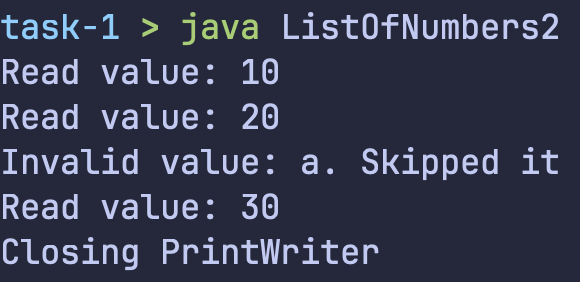
\includegraphics[width=0.5\textwidth]{images/task-1.png}
  \caption{Пример работы программы}
  \label{fig:task-1-2}
\end{figure}

\subsection*{Упражнение 2. Знакомство с классом BufferedReader}

В данном упражнении необходимо реализовать функцию \textit{main}, в которой, с
помощью уже существующего метода \textit{countTokens}, будет происходить вывод
количества вхождений слова, которое вводит пользователь.

На рисунке \ref{fig:task-2-1} представлен исходный код получившейся функции
\textit{main}. Сначала проверяется количество переданных аргументов. Если
аргументов передано не было, пользователю сообщается об ошибке. Затем первый
аргумент используется в качестве имени файла.

Для считывания пользовательского ввода используется \textit{BufferReader} из
стандартной библиотеки Java. Считывание происходит построчно, и при считывании
проверяется, не равна ли входная строка значению q. Если равна, то работа
программы прекращается. При вводе любого другого слова выводится количество
вхождений данного слова в переданный файл.

\begin{figure}[H]
  \begin{minted}{java}
    public static void main(String[] args) {
        if (args.length < 1) {
            System.out.println("Expected filename");
            System.exit(-1);
        }

        String file = args[0];
        FileScanInteractive scanner = new FileScanInteractive();

        try (
            BufferedReader br = new BufferedReader(
                new InputStreamReader(System.in)
            )
        ) {
            while (true) {
                System.out.print("Enter the search string or q to exit: ");
                String line = br.readLine().trim();
                if (line.equalsIgnoreCase("q")) {
                    break;
                }

                System.out.printf(
                    "Count of %s in file: %d\n",
                    line,
                    scanner.countTokens(file, line)
                );
            }
        } catch (IOException e) {
            System.err.println("Error: " + e.getMessage());
        }
    }
  \end{minted}
  \caption{Исходный код функции \textit{main}}
  \label{fig:task-2-1}
\end{figure}

На рисунке \ref{fig:task-2-2} приведен пример работы программы. Как видно,
программа выводит верное количество вхождений. Это можно проверить, пересчитав
количество вхождений с помощью других инструментов.

\begin{figure}[H]
  \centering
  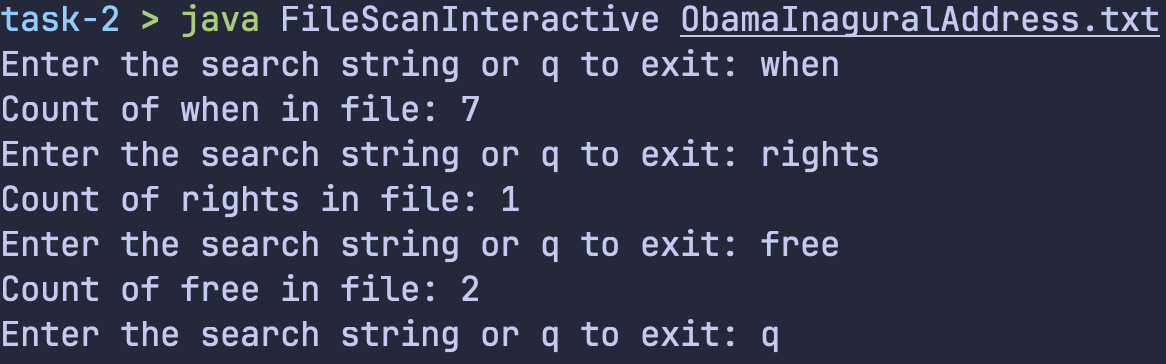
\includegraphics[width=0.7\textwidth]{images/task-2.png}
  \caption{Пример работы программы}
  \label{fig:task-2-2}
\end{figure}

\section*{Заключение}

В данной лабораторной работе были разработаны приложении, использующие потоки
ввода и вывода для считывания информации от пользователя и вывода информации.
Цель, поставленная в начале работы, достигнута, задачи выполнены.

\end{document}
